%%%%%%%%%%%%%%%%%%%%%%%%%%%%%%%%%%%%%%%%%%%%%%%%%%%%%%%%%%%%%%%%%%%%%%%%%%%%%%%%
%% Plantilla de memoria en LaTeX para la ETSIT - Universidad Rey Juan Carlos
%%
%% Por Gregorio Robles <grex arroba gsyc.urjc.es>
%%     Grupo de Sistemas y Comunicaciones
%%     Escuela Técnica Superior de Ingenieros de Telecomunicación
%%     Universidad Rey Juan Carlos
%% (muchas ideas tomadas de Internet, colegas del GSyC, antiguos alumnos...
%%  etc. Muchas gracias a todos)
%%
%% La última versión de esta plantilla está siempre disponible en:
%%     https://github.com/gregoriorobles/plantilla-memoria
%%
%% Para obtener PDF, ejecuta en la shell:
%%   make
%% (las imágenes deben ir en PNG o JPG)

%%%%%%%%%%%%%%%%%%%%%%%%%%%%%%%%%%%%%%%%%%%%%%%%%%%%%%%%%%%%%%%%%%%%%%%%%%%%%%%%

\documentclass[a4paper, 12pt]{book}
%\usepackage[T1]{fontenc}

\usepackage[a4paper, left=2.5cm, right=2.5cm, top=3cm, bottom=3cm]{geometry}
\usepackage{times}
\usepackage[utf8]{inputenc}
\usepackage[spanish]{babel} % Comenta esta línea si tu memoria es en inglés
\usepackage{url}
%\usepackage[dvipdfm]{graphicx}
\usepackage{graphicx}
\usepackage{float}  %% H para posicionar figuras
\usepackage[nottoc, notlot, notlof, notindex]{tocbibind} %% Opciones de índice
\usepackage{latexsym}  %% Logo LaTeX

\title{Memoria del Proyecto}
\author{Daniel Hervás Rodao}

\renewcommand{\baselinestretch}{1.5}  %% Interlineado

\begin{document}

\renewcommand{\refname}{Bibliografía}  %% Renombrando
\renewcommand{\appendixname}{Apéndice}

%%%%%%%%%%%%%%%%%%%%%%%%%%%%%%%%%%%%%%%%%%%%%%%%%%%%%%%%%%%%%%%%%%%%%%%%%%%%%%%%
% PORTADA

\begin{titlepage}
\begin{center}

\includegraphics[scale=0.8]{img/URJ_logo_Color_POS.png}

\vspace{1.75cm}

\Large
GRADO EN INGENIERÍA EN TELEMÁTICA

\vspace{0.4cm}

\large
Curso Académico 2021/2022

\vspace{0.8cm}

Trabajo Fin de Grado

\vspace{2.5cm}

\LARGE
GAMIFICACIÓN DE PLATAFORMA UNIBOTICS

\vspace{4cm}

\large
Autor : Daniel Hervás Rodao \\
Tutor : José María Cañas Plaza \\
Co-Tutor : David Roldán Álvarez
\end{center}
\end{titlepage}

\newpage
\mbox{}
\thispagestyle{empty} % para que no se numere esta pagina


%%%%%%%%%%%%%%%%%%%%%%%%%%%%%%%%%%%%%%%%%%%%%%%%%%%%%%%%%%%%%%%%%%%%%%%%%%%%%%%%
%%%% Para firmar
\clearpage
\pagenumbering{gobble}
\chapter*{}

\vspace{-4cm}
\begin{center}
\LARGE
\textbf{Trabajo Fin de Grado}

\vspace{1cm}
\large
Gamificación de la Plataforma Unibotics

\vspace{1cm}
\large
\textbf{Autor :} Daniel Hervás Rodao \\
\textbf{Tutor :} José María Cañas Plaza
\textbf{Co-Tutor :} David Roldán Álvarez

\end{center}

\vspace{1cm}
La defensa del presente Proyecto Fin de Carrera se realizó el día \qquad$\;\,$ de \qquad\qquad\qquad\qquad \newline de 202X, siendo calificada por el siguiente tribunal:


\vspace{0.5cm}
\textbf{Presidente:}

\vspace{1.2cm}
\textbf{Secretario:}

\vspace{1.2cm}
\textbf{Vocal:}


\vspace{1.2cm}
y habiendo obtenido la siguiente calificación:

\vspace{1cm}
\textbf{Calificación:}


\vspace{1cm}
\begin{flushright}
Fuenlabrada, a \qquad$\;\,$ de \qquad\qquad\qquad\qquad de 202X
\end{flushright}

%%%%%%%%%%%%%%%%%%%%%%%%%%%%%%%%%%%%%%%%%%%%%%%%%%%%%%%%%%%%%%%%%%%%%%%%%%%%%%%%
%%%% Dedicatoria

\chapter*{}
\pagenumbering{Roman} % para comenzar la numeracion de paginas en numeros romanos
\begin{flushright}
\textit{Dedicado a \\
mi familia / mi abuelo / mi abuela}
\end{flushright}

%%%%%%%%%%%%%%%%%%%%%%%%%%%%%%%%%%%%%%%%%%%%%%%%%%%%%%%%%%%%%%%%%%%%%%%%%%%%%%%%
%%%% Agradecimientos

\chapter*{Agradecimientos}
%\addcontentsline{toc}{chapter}{Agradecimientos} % si queremos que aparezca en el índice
\markboth{AGRADECIMIENTOS}{AGRADECIMIENTOS} % encabezado 

Aquí vienen los agradecimientos\ldots Aunque está bien acordarse de la pareja, no hay que olvidarse de dar las gracias a tu madre, que aunque a veces no lo parezca disfrutará tanto de tus logros como tú\ldots 
Además, la pareja quizás no sea para siempre, pero tu madre sí.

%%%%%%%%%%%%%%%%%%%%%%%%%%%%%%%%%%%%%%%%%%%%%%%%%%%%%%%%%%%%%%%%%%%%%%%%%%%%%%%%
%%%% Resumen

\chapter*{Resumen}
%\addcontentsline{toc}{chapter}{Resumen} % si queremos que aparezca en el índice
\markboth{RESUMEN}{RESUMEN} % encabezado

Aquí viene un resumen del proyecto.
Ha de constar de tres o cuatro párrafos, donde se presente de manera clara y concisa de qué va el proyecto. 
Han de quedar respondidas las siguientes preguntas:

\begin{itemize}
  \item ¿De qué va este proyecto? ¿Cuál es su objetivo principal?
  \item ¿Cómo se ha realizado? ¿Qué tecnologías están involucradas?
  \item ¿En qué contexto se ha realizado el proyecto? ¿Es un proyecto dentro de un marco general?
\end{itemize}

Lo mejor es escribir el resumen al final.

%%%%%%%%%%%%%%%%%%%%%%%%%%%%%%%%%%%%%%%%%%%%%%%%%%%%%%%%%%%%%%%%%%%%%%%%%%%%%%%%
%%%% Resumen en inglés

\chapter*{Summary}
%\addcontentsline{toc}{chapter}{Summary} % si queremos que aparezca en el índice
\markboth{SUMMARY}{SUMMARY} % encabezado

Here comes a translation of the ``Resumen'' into English. 
Please, double check it for correct grammar and spelling.
As it is the translation of the ``Resumen'', which is supposed to be written at the end, this as well should be filled out just before submitting.


%%%%%%%%%%%%%%%%%%%%%%%%%%%%%%%%%%%%%%%%%%%%%%%%%%%%%%%%%%%%%%%%%%%%%%%%%%%%%%%%
%%%%%%%%%%%%%%%%%%%%%%%%%%%%%%%%%%%%%%%%%%%%%%%%%%%%%%%%%%%%%%%%%%%%%%%%%%%%%%%%
% ÍNDICES %
%%%%%%%%%%%%%%%%%%%%%%%%%%%%%%%%%%%%%%%%%%%%%%%%%%%%%%%%%%%%%%%%%%%%%%%%%%%%%%%%

% Las buenas noticias es que los índices se generan automáticamente.
% Lo único que tienes que hacer es elegir cuáles quieren que se generen,
% y comentar/descomentar esa instrucción de LaTeX.

%%%% Índice de contenidos
\tableofcontents 
%%%% Índice de figuras
\cleardoublepage
%\addcontentsline{toc}{chapter}{Lista de figuras} % para que aparezca en el indice de contenidos
\listoffigures % indice de figuras
%%%% Índice de tablas
%\cleardoublepage
%\addcontentsline{toc}{chapter}{Lista de tablas} % para que aparezca en el indice de contenidos
%\listoftables % indice de tablas


%%%%%%%%%%%%%%%%%%%%%%%%%%%%%%%%%%%%%%%%%%%%%%%%%%%%%%%%%%%%%%%%%%%%%%%%%%%%%%%%
%%%%%%%%%%%%%%%%%%%%%%%%%%%%%%%%%%%%%%%%%%%%%%%%%%%%%%%%%%%%%%%%%%%%%%%%%%%%%%%%
% INTRODUCCIÓN %
%%%%%%%%%%%%%%%%%%%%%%%%%%%%%%%%%%%%%%%%%%%%%%%%%%%%%%%%%%%%%%%%%%%%%%%%%%%%%%%%

\cleardoublepage
\chapter{Introducción}
\label{sec:intro} % etiqueta para poder referenciar luego en el texto con ~\ref{sec:intro}
\pagenumbering{arabic} % para empezar la numeración de página con números

El TFG que será descrito a continuación se ha desarrollado en la plataforma \textit{Unibotics} de la asociación \textit{JdeRobot}\footnote{\url{https://jderobot.github.io}}, orientado al aprendizaje de robótica para estudiantes universitarios. El principal motivo de este proyecto es la introducción de técnicas de gamificación para los diferentes ejercicios contenidos la plataforma, así como añadir nuevos.

En este capítulo introductorio se introducirá el contexto en el que se desarrolla el trabajo, así como los motivos que han motivado a llevarlo a cabo.

El campo de la robótica es muy amplio, en concreto, este TFG se encuentra en el marco de la robótica educativa, destinada a la enzeñanza de la misma. 

\section{Robótica}
\label{sec:robotica}

Los avances en computación de las últimas décadas han sido el impulso que ha permitido la creación de máquinas muy cercanas al ideal de autonomía que se ha perseguido siempre. La robótica está muy relacionada no solo con la rama de la ingeniería, si no, que involucra conocimientos de matemáticas y física para el desarrollos de máquinas autónomas. Uno de los objetivos principales de la robótica es el de facilitar tareas de la vida diaria al ser humano, incluso, en algunas ocasiones, sustituir al ser humano.

La inteligencia artificial, también está muy ligada al campo de la robótica. Los avances en este campo permiten desarrollar sistemas capaces de tener una cierta memoria útil para realizar una serie de funciones.

En 1950 la robótica experimenta un gran desarrollo. Esto se debe a los grandes avances en relación a la potencia y complejidad computacional. El acoplamiento mecánico empezó a sustituirse por sistemas eléctricos. Tal es el grado de desarrollo que se empiezan a generar sistemas de control automático consistentes en máquinas de estado secuencial.

Un claro ejemplo de este gran impluso es la implementación de robots en la industria automovilística, capaces de realizar tareas repetitivas, y que conllevan un gran riesgo para las personas (Figura 1.1).


\begin{figure}[H]
	\centering
    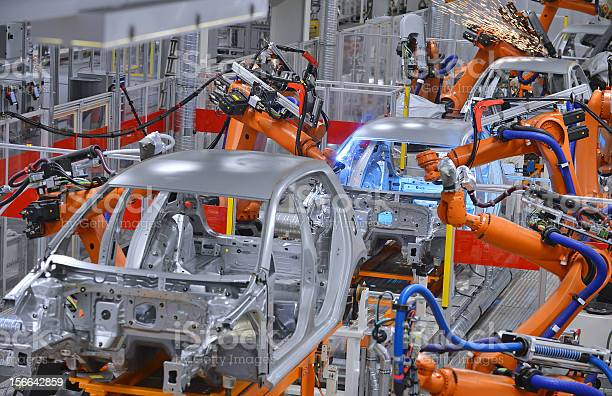
\includegraphics[width=8cm, keepaspectratio]{img/brazo}
    \caption{Brazo robótico.}
    \label{figura:brazo_robotico}
\end{figure}

En la actualidad, cada vez son más populares los coches autónomos. Es un campo muy amplio que cuenta con un gran número de posibilidades. Alguna de estas posibilidades serían los coches con conducción autónoma de \textit{Tesla}  (Figura 1.2) o los coches con aparcamiento autónomo que están desarrollando un gran número de compañías en la actualidad.

\begin{figure}[H]
	\centering
    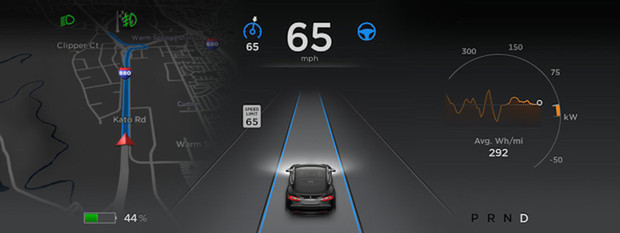
\includegraphics[width=8cm, keepaspectratio]{img/coche}
    \caption{Coche autónomo.}
    \label{figura:coche_autonomo}
\end{figure}

Otro campo de la aplicación de la robótica es la medicina, donde existen robots capaces de filtrar las vibraciones naturales del humano para proporcionarle una gran precisión y seguridad, un claro ejemplo es el robot DaVinci (Figura 1.3). Adicionalmente, hay robots capaces de mantener una estabilidad la estabilidad necesaria para caminar sobre dos piernas robóticas, como es el robot ATRIAS (Figura 1.4).

\begin{figure}[H]
  \centering
  \begin{minipage}[b]{0.4\textwidth}
    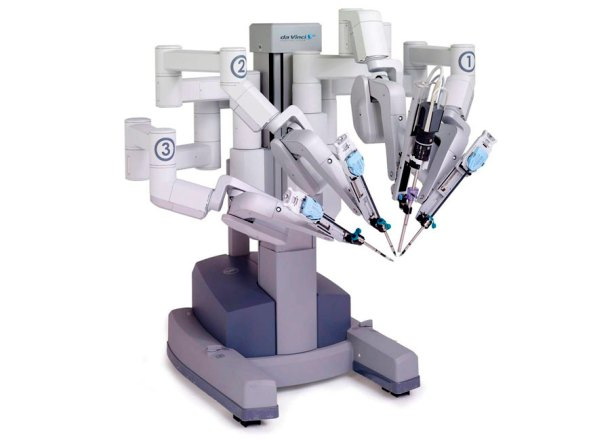
\includegraphics[width=\textwidth]{img/davinci}
    \caption{Robot DaVinci.}
    \label{figura:robot_davinci}
  \end{minipage}
  \hfill
  \begin{minipage}[b]{0.4\textwidth}
    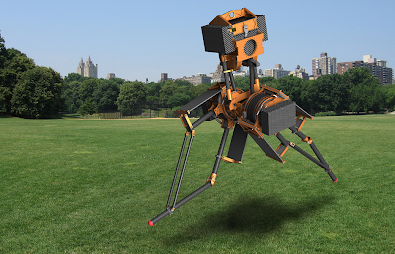
\includegraphics[width=\textwidth]{img/atrias}
    \caption{Robot ATRIAS.}
    \label{figura:robot_atrias}
  \end{minipage}
\end{figure}

En el ámbito militar, existen robots capaces de sustituir a una persona en el a la hora de realizar tareas de gran peligro como la desactivación de bombas y la entrada en zonas contaminadas (Figura 1.5).

\begin{figure}[H]
	\centering
    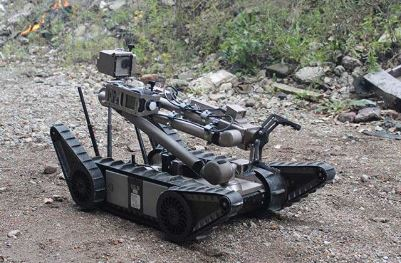
\includegraphics[width=8cm]{img/robot_militar}
    \caption{Robot militar.}
    \label{figura:coche_autonomo}
\end{figure}

\section{Componentes robóticas}
\label{subsec:componentes roboticas}

Todo robot está formado por dos componentes: el \textit{software}, encargado de proporcionar la inteligencia al robot, el más importante, y, el \textit{hardware} encargado de proporcionar la estructura física del robot.

Con al gran auge de la robótica han surgido numerosas plataformas que proporcionan herramientas que simplifican el desarrollo de software robótico, esto son los denominados \textit{middlewares} robóticos.

Durante el desarrollo de software robótico es preciso realizar una serie de pruebas para comprobar el funcionamiento del código y depurar errores, por lo que se necesitan simuladores que nos proporcionen un entorno cercano a la realidad previa al ensamblado del robot.

\subsection{Middlewares robóticos}
\label{subsec:middlewares}

Un \textit{middleware} robótico es un \textit{framework} que proporciona una serie de herramientas que facilitan el desarrollo de software para robots. Proporciona los servicios necesarios para soportar y simplificar aplicaciones complejas y distribuidas. Para el control de los sensores y actuadores de los robots, los \textit{middlewares} proporcionan \textit{drivers}, APIs, etc.

El \textit{middleware} robótico más generalizado es ROS\footnote{\url{https://www.ros.org/}}
 (\textit{Robotics Operating System}). \textit{Robotics Operating System} fue desarrollado en 2007 por el Laboratorio de Inteligencia Artificial de Stanford para dar soporte a sus proyectos. A pesar de no ser un sistema operativo, ROS proporciona tales servicios coko la abstracción \textit{hardware}, mecanismos de comunicación entre prosesos, el control de dispositivos de bajo nivel y el mantenimiento de paquetes. \textit{Robotics Operating System} fue desarrollado para sistemas UNIX, aunque en la actualidad está siendo adaptado para su funcionamiento en sistemas operativos como Fedora, Mac OS X, Arch, Gentoo, OpenSUSE, Slackware, Debian o Microsoft Windows.

\subsection{Simuladores robóticos}
\label{subsec:simuladores}

El surgimiento de estos \textit{softwares} robóticos está condicionado por la necesidad de realizar pruebas durante el desarrollo del \textit{software} para la detección y depuración de posibles errores antes de llevarlo a un robot real debido al gran coste que suponen.

El simulador más generalizado en la actualidad es \textit{Gazebo}\footnote{\url{http://gazebosim.org/}}. Su popularidad se debe a su robusto motor de físicas, sus gráficos de alta calidad y su amplio catálogo de robots y escenarios. Es una herramienta de código abierto integrada con ROS, por lo que permite ejecutar \textit{software} robótico en un escenario simulado (Figura 1.6).

\begin{figure}[H]
	\centering
    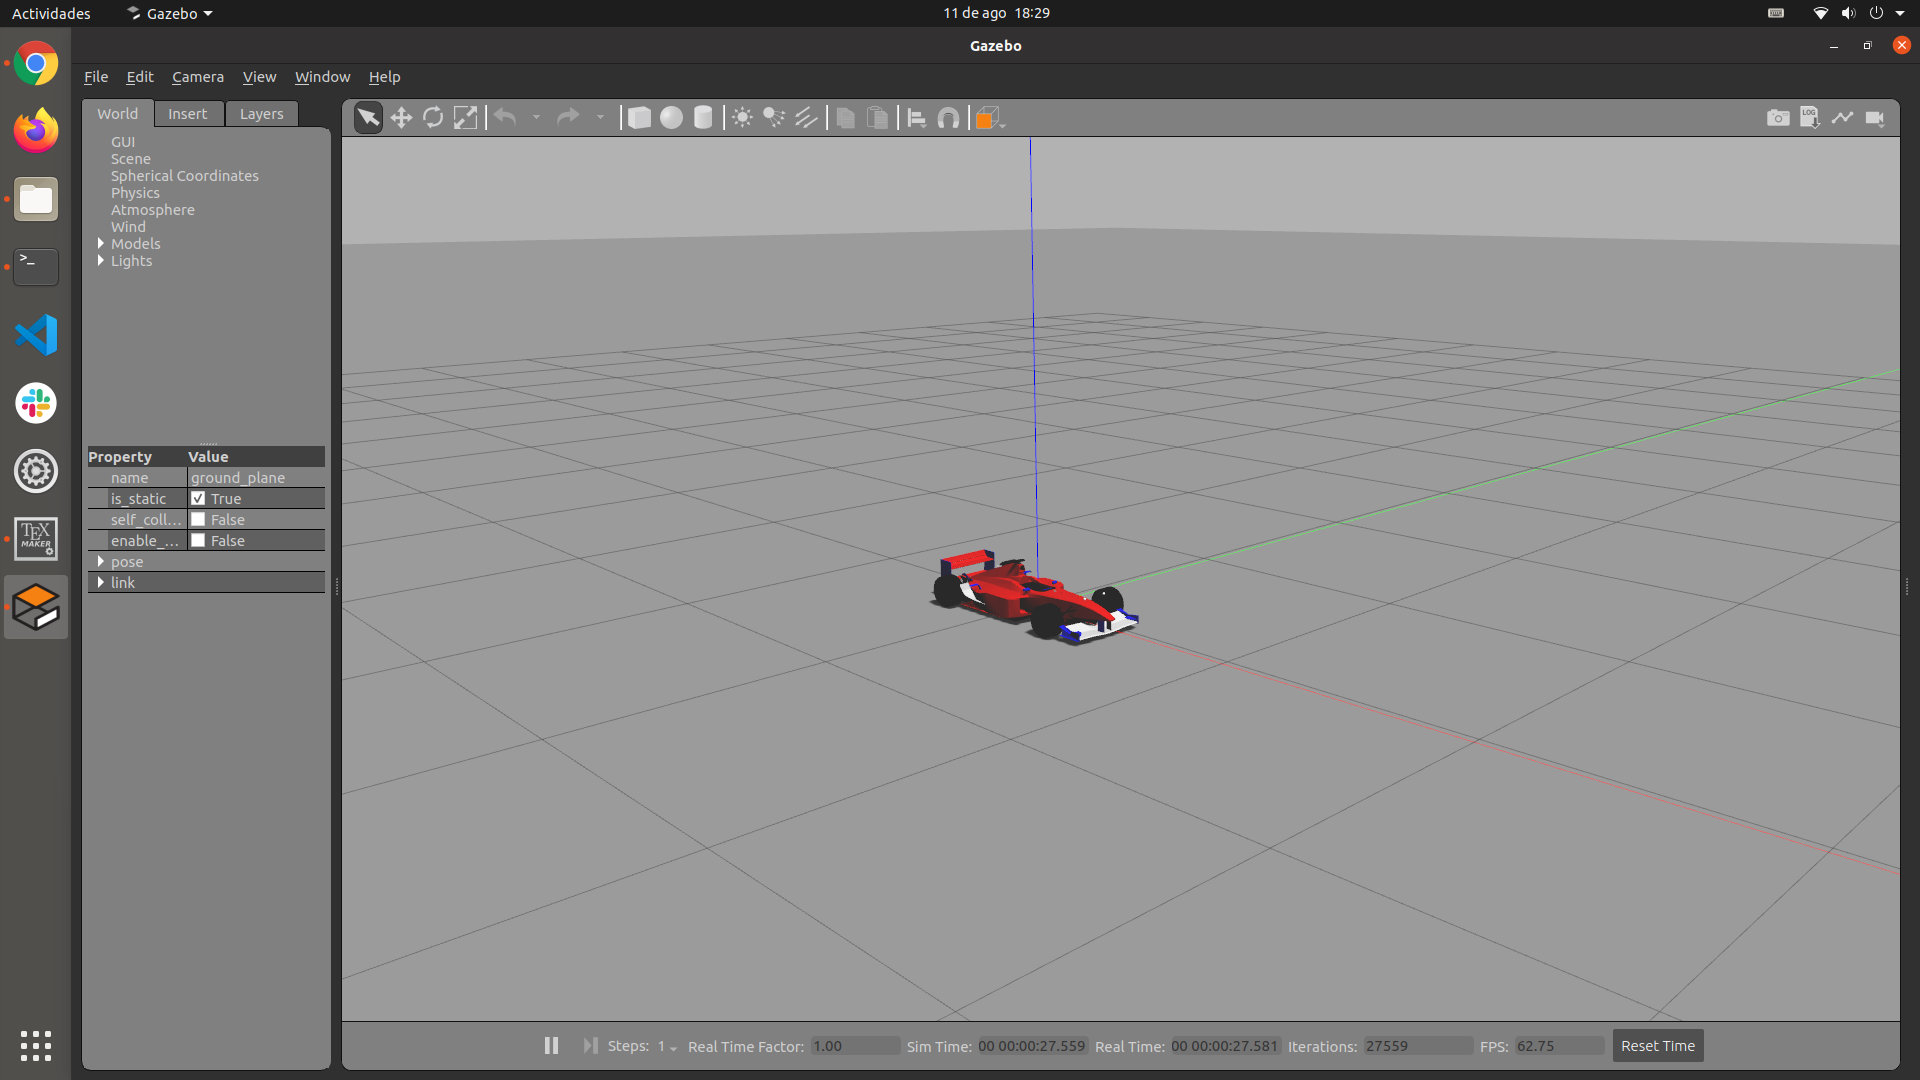
\includegraphics[width=\textwidth]{img/gazebo}
    \caption{Simulador Gazebo.}
    \label{figura:simulador_gazebo}
\end{figure}

\section{Robótica educativa}
\label{sec:robotica educativa}

La robótica educativa proporciona a los estudiantes la infraestructura para la construcción y programación de un robot, pero, además de la enseñanza robótica,
estos entornos van más allá, ofrenciendo la capacidad para el alumno de adquirir un pensamiento lógico. También, contribuye en la adquisición de una mentalidad resolutiva y al enriquecimiento de la cultura científica de los alumnos. Este método de educación con la robótica como objeto de enseñanza se denomina el método STEAM (Science, Technology, Engineering and Matemathics).

Como se ha comentado, para llevar a cabo este método de educación es necesaria una infraestructura, como puede ser LEGO Mindstroms, un kit de robótica que es capaz de aumentras la capacidad de pensamiento de los alumnos.

Dentro de la robótica educativa, es preciso enfatizar la plataforma \textit{Unibotics} en la que se desarrolla el presente proyecto. Esta plataforma es un proyecto internacional que ofrece material para la enseñanza de robótica en las aulas. \textit{Unibotics} proporciona una infraestructura software en conjunto a una colección de ejercicios, cada uno con el material teórico correspondiente para su resolución.

%%%%%%%%%%%%%%%%%%%%%%%%%%%%%%%%%%%%%%%%%%%%%%%%%%%%%%%%%%%%%%%%%%%%%%%%%%%%%%%%
%%%%%%%%%%%%%%%%%%%%%%%%%%%%%%%%%%%%%%%%%%%%%%%%%%%%%%%%%%%%%%%%%%%%%%%%%%%%%%%%
% OBJETIVOS %
%%%%%%%%%%%%%%%%%%%%%%%%%%%%%%%%%%%%%%%%%%%%%%%%%%%%%%%%%%%%%%%%%%%%%%%%%%%%%%%%

\cleardoublepage % empezamos en página impar
\chapter{Objetivos} % título del capítulo (se muestra)
\label{chap:objetivos} % identificador del capítulo (no se muestra, es para poder referenciarlo)

\section{Objetivo general} % título de sección (se muestra)
\label{sec:objetivo-general} % identificador de sección (no se muestra, es para poder referenciarla)

Aquí vendría el objetivo general en una frase:
Mi trabajo fin de grado consiste en crear de una herramienta de análisis de los comentarios jocosos en repositorios de software libre alojados en la plataforma GitHub.

Recuerda que los objetivos siempre vienen en infinitivo.


\section{Objetivos específicos}
\label{sec:objetivos-especificos}

Los objetivos específicos se pueden entender como las tareas en las que se ha desglosado el objetivo general.
Y, sí, también vienen en infinitivo.


\section{Planificación temporal}
\label{sec:planificacion-temporal}

A mí me gusta que aquí pongáis una descripción de lo que os ha llevado realizar el trabajo.
Hay gente que añade un diagrama de GANTT.
Lo importante es que quede claro cuánto tiempo llevas (tiempo natural, p.ej., 6 meses) y a qué nivel de esfuerzo (p.ej., principalmente los fines de semana).


%%%%%%%%%%%%%%%%%%%%%%%%%%%%%%%%%%%%%%%%%%%%%%%%%%%%%%%%%%%%%%%%%%%%%%%%%%%%%%%%
%%%%%%%%%%%%%%%%%%%%%%%%%%%%%%%%%%%%%%%%%%%%%%%%%%%%%%%%%%%%%%%%%%%%%%%%%%%%%%%%
% ESTADO DEL ARTE %
%%%%%%%%%%%%%%%%%%%%%%%%%%%%%%%%%%%%%%%%%%%%%%%%%%%%%%%%%%%%%%%%%%%%%%%%%%%%%%%%

\cleardoublepage
\chapter{Estado del arte}
\label{chap:estado}

Descripción de las tecnologías que utilizas en tu trabajo. 
Con dos o tres párrafos por cada tecnología, vale. 
Se supone que aquí viene todo lo que no has hecho tú.

Puedes citar libros, como el de Bonabeau et al., sobre procesos estigmérgicos~\cite{bonabeau:_swarm}. 
Me encantan los procesos estigmérgicos.
Deberías leer más sobre ellos.
Pero quizás no ahora, que tenemos que terminar la memoria para sacarnos por fin el título.
Nota que el \~ \ añade un espacio en blanco, pero no deja que exista un salto de línea. 
Imprescindible ponerlo para las citas.

Citar es importantísimo en textos científico-técnicos. 
Porque no partimos de cero.
Es más, partir de cero es de tontos; lo suyo es aprovecharse de lo ya existente para construir encima y hacer cosas más sofisticadas.
¿Dónde puedo encontrar textos científicos que referenciar?
Un buen sitio es Google Scholar\footnote{\url{http://scholar.google.com}}.
Por ejemplo, si buscas por ``stigmergy libre software'' para encontrar trabajo sobre software libre y el concepto de \emph{estigmergia} (¿te he comentado que me gusta el concepto de estigmergia ya?), encontrarás un artículo que escribí hace tiempo cuyo título es ``Self-organized development in libre software: a model based on the stigmergy concept''.
Si pulsas sobre las comillas dobles (entre la estrella y el ``citado por ...'', justo debajo del extracto del resumen del artículo, te saldrá una ventana emergente con cómo citar.
Abajo a la derecha, aparece un enlace BibTeX.
Púlsalo y encontrarás la referencia en formato BibTeX, tal que así:

{\footnotesize
\begin{verbatim}
@inproceedings{robles2005self,
  title={Self-organized development in libre software:
         a model based on the stigmergy concept},
  author={Robles, Gregorio and Merelo, Juan Juli\'an 
          and Gonz\'alez-Barahona, Jes\'us M.},
  booktitle={ProSim'05},
  year={2005}
}
\end{verbatim}
}

Copia el texto en BibTeX y pégalo en el fichero \texttt{memoria.bib}, que es donde están las referencias bibliográficas.
Para incluir la referencia en el texto de la memoria, deberás citarlo, como hemos hecho antes con~\cite{bonabeau:_swarm}, lo que pasa es que en vez de el identificador de la cita anterior (bonabeau:\_swarm), tendrás que poner el nuevo (robles2005self).
Compila el fichero \texttt{memoria.tex} (\texttt{pdflatex memoria.tex}), añade la bibliografía (\texttt{bibtex memoria.aux}) y vuelve a compilar \texttt{memoria.tex} (\texttt{pdflatex memoria.tex})\ldots y \emph{voilà} ¡tenemos una nueva cita~\cite{robles2005self}!

También existe la posibilidad de poner notas al pie de página, por ejemplo, una para indicarte que visite la página del GSyC\footnote{\url{http://gsyc.es}}.



\section{Sección 1} 
\label{sec:seccion1}

Hemos hablado de cómo incluir figuras.
Pero no hemos dicho nada de tablas.
A mí me gustan las tablas.
Mucho.
Aquí un ejemplo de tabla, la Tabla~\ref{tabla:ejemplo} (siento ser pesado, pero nota cómo he puesto la referencia).

\begin{table}
 \begin{center}
  \begin{tabular}{ | l | c | r |} % tenemos tres colummnas, la primera alineada a la izquierda (l), la segunda al centro (c) y la tercera a la derecha (r). El | indica que entre las columnas habrá una línea separadora.
    \hline
    Uno & 2 & 3 \\ \hline % el hline nos da una línea vertical
    Cuatro & 5 & 6 \\ \hline
    Siete & 8 & 9 \\
    \hline
  \end{tabular}
  \label{tabla:ejemplo}
  \caption{Ejemplo de tabla. Aquí viene una pequeña descripción (el \emph{caption}) del contenido de la tabla. Si la tabla no es autoexplicativa, siempre viene bien aclararla aquí.}
 \end{center}
\end{table}



%%%%%%%%%%%%%%%%%%%%%%%%%%%%%%%%%%%%%%%%%%%%%%%%%%%%%%%%%%%%%%%%%%%%%%%%%%%%%%%%
%%%%%%%%%%%%%%%%%%%%%%%%%%%%%%%%%%%%%%%%%%%%%%%%%%%%%%%%%%%%%%%%%%%%%%%%%%%%%%%%
% DISEÑO E IMPLEMENTACIÓN %
%%%%%%%%%%%%%%%%%%%%%%%%%%%%%%%%%%%%%%%%%%%%%%%%%%%%%%%%%%%%%%%%%%%%%%%%%%%%%%%%

\cleardoublepage
\chapter{Diseño e implementación}

Aquí viene todo lo que has hecho tú (tecnológicamente). 
Puedes entrar hasta el detalle. 
Es la parte más importante de la memoria, porque describe lo que has hecho tú.
Eso sí, normalmente aconsejo no poner código, sino diagramas.

\section{Arquitectura general} 
\label{sec:arquitectura}

Si tu proyecto es un software, siempre es bueno poner la arquitectura (que es cómo se estructura tu programa a ``vista de pájaro'').

Por ejemplo, puedes verlo en la figura~\ref{fig:arquitectura}.
\LaTeX \ pone las figuras donde mejor cuadran. 
Y eso quiere decir que quizás no lo haga donde lo hemos puesto\ldots
Eso no es malo.
A veces queda un poco raro, pero es la filosofía de \LaTeX: tú al contenido, que yo me encargo de la maquetación.

\begin{figure}
  \centering
  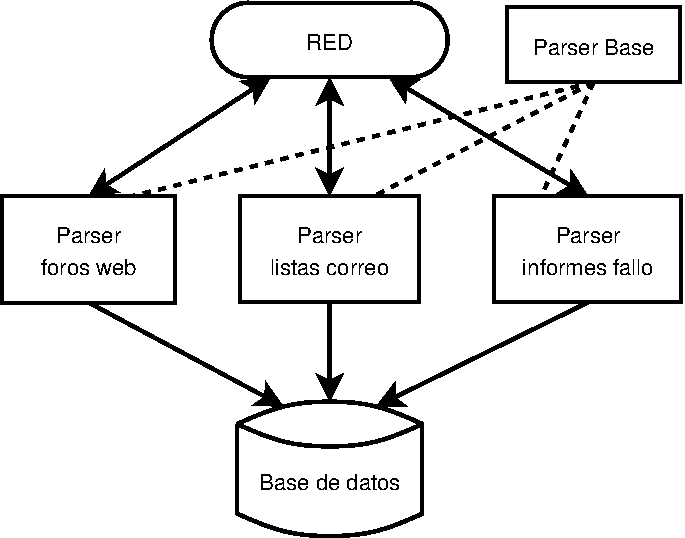
\includegraphics[width=9cm, keepaspectratio]{img/arquitectura.png}
  \caption{Estructura del parser básico.}\label{fig:arquitectura}
\end{figure}

\begin{figure}
    \centering
    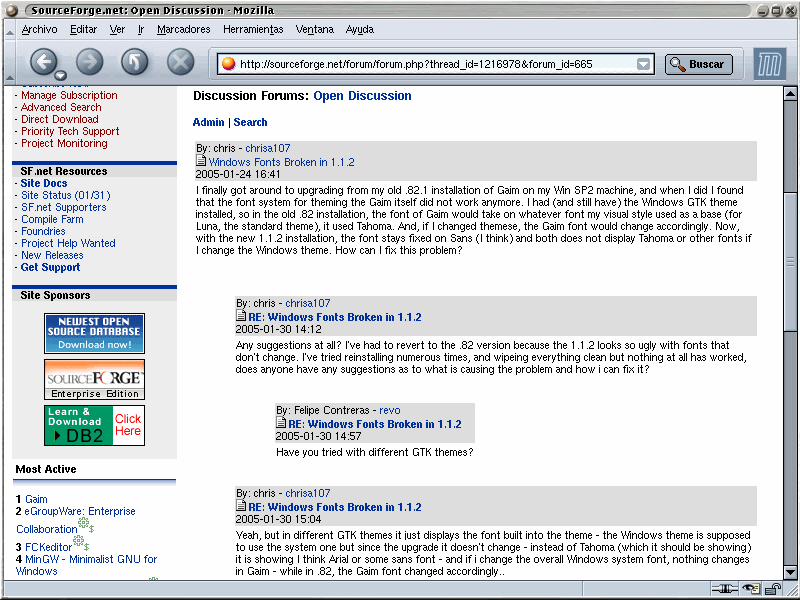
\includegraphics[bb=0 0 800 600, width=12cm, keepaspectratio]{img/foro1}
    \caption{Página con enlaces a hilos}\label{fig:_arquitectura}
\end{figure}

 
Recuerda que toda figura que añadas a tu memoria debe ser explicada.
Sí, aunque te parezca evidente lo que se ve en la figura~\ref{fig:arquitectura}, la figura en sí solamente es un apoyo a tu texto.
Así que explica lo que se ve en la figura, haciendo referencia a la misma tal y como ves aquí.
Por ejemplo: En la figura~\ref{fig:arquitectura} se puede ver que la estructura del \emph{parser} básico, que consta de seis componentes diferentes: los datos se obtienen de la red, y según el tipo de dato, se pasará a un \emph{parser} específico y bla, bla, bla\ldots

Si utilizas una base de datos, no te olvides de incluir también un diagrama de entidad-relación.


%%%%%%%%%%%%%%%%%%%%%%%%%%%%%%%%%%%%%%%%%%%%%%%%%%%%%%%%%%%%%%%%%%%%%%%%%%%%%%%%
%%%%%%%%%%%%%%%%%%%%%%%%%%%%%%%%%%%%%%%%%%%%%%%%%%%%%%%%%%%%%%%%%%%%%%%%%%%%%%%%
% EXPERIMENTOS Y VALIDACIÓN %
%%%%%%%%%%%%%%%%%%%%%%%%%%%%%%%%%%%%%%%%%%%%%%%%%%%%%%%%%%%%%%%%%%%%%%%%%%%%%%%%

\cleardoublepage
\chapter{Experimentos y validación}

Este capítulo se introdujo como requisito en 2019. 
Describe los experimentos y casos de test que tuviste que implementar para validar tus resultados. 
Incluye también los resultados de validación que permiten afirmar que tus resultados son correctos. 


%%%%%%%%%%%%%%%%%%%%%%%%%%%%%%%%%%%%%%%%%%%%%%%%%%%%%%%%%%%%%%%%%%%%%%%%%%%%%%%%
%%%%%%%%%%%%%%%%%%%%%%%%%%%%%%%%%%%%%%%%%%%%%%%%%%%%%%%%%%%%%%%%%%%%%%%%%%%%%%%%
% RESULTADOS %
%%%%%%%%%%%%%%%%%%%%%%%%%%%%%%%%%%%%%%%%%%%%%%%%%%%%%%%%%%%%%%%%%%%%%%%%%%%%%%%%

\cleardoublepage
\chapter{Resultados}

En este capítulo se incluyen los resultados de tu trabajo fin de grado.

Si es una herramienta de análisis lo que has realizado, aquí puedes poner ejemplos de haberla utilizado para que se vea su utilidad.


%%%%%%%%%%%%%%%%%%%%%%%%%%%%%%%%%%%%%%%%%%%%%%%%%%%%%%%%%%%%%%%%%%%%%%%%%%%%%%%%
%%%%%%%%%%%%%%%%%%%%%%%%%%%%%%%%%%%%%%%%%%%%%%%%%%%%%%%%%%%%%%%%%%%%%%%%%%%%%%%%
% CONCLUSIONES %
%%%%%%%%%%%%%%%%%%%%%%%%%%%%%%%%%%%%%%%%%%%%%%%%%%%%%%%%%%%%%%%%%%%%%%%%%%%%%%%%

\cleardoublepage
\chapter{Conclusiones}
\label{chap:conclusiones}


\section{Consecución de objetivos}
\label{sec:consecucion-objetivos}

Esta sección es la sección espejo de las dos primeras del capítulo de objetivos, donde se planteaba el objetivo general y se elaboraban los específicos.

Es aquí donde hay que debatir qué se ha conseguido y qué no. 
Cuando algo no se ha conseguido, se ha de justificar, en términos de qué problemas se han encontrado y qué medidas se han tomado para mitigar esos problemas.

Y si has llegado hasta aquí, siempre es bueno pasarle el corrector ortográfico, que las erratas quedan fatal en la memoria final.
Para eso, en Linux tenemos aspell, que se ejecuta de la siguiente manera desde la línea de \emph{shell}:

\begin{verbatim}
  aspell --lang=es_ES -c memoria.tex
\end{verbatim}

\section{Aplicación de lo aprendido}
\label{sec:aplicacion}

Aquí viene lo que has aprendido durante el Grado/Máster y que has aplicado en el TFG/TFM. Una buena idea es poner las asignaturas más relacionadas y comentar en un párrafo los conocimientos y habilidades puestos en práctica.

\begin{enumerate}
  \item a
  \item b
\end{enumerate}


\section{Lecciones aprendidas}
\label{sec:lecciones_aprendidas}

Aquí viene lo que has aprendido en el Trabajo Fin de Grado/Máster.

\begin{enumerate}
  \item Aquí viene uno.
  \item Aquí viene otro.
\end{enumerate}


\section{Trabajos futuros}
\label{sec:trabajos_futuros}

Ningún proyecto ni software se termina, así que aquí vienen ideas y funcionalidades que estaría bien tener implementadas en el futuro.

Es un apartado que sirve para dar ideas de cara a futuros TFGs/TFMs.


%%%%%%%%%%%%%%%%%%%%%%%%%%%%%%%%%%%%%%%%%%%%%%%%%%%%%%%%%%%%%%%%%%%%%%%%%%%%%%%%
%%%%%%%%%%%%%%%%%%%%%%%%%%%%%%%%%%%%%%%%%%%%%%%%%%%%%%%%%%%%%%%%%%%%%%%%%%%%%%%%
% APÉNDICE(S) %
%%%%%%%%%%%%%%%%%%%%%%%%%%%%%%%%%%%%%%%%%%%%%%%%%%%%%%%%%%%%%%%%%%%%%%%%%%%%%%%%

\cleardoublepage
\appendix
\chapter{Manual de usuario}
\label{app:manual}

Esto es un apéndice.
Si has creado una aplicación, siempre viene bien tener un manual de usuario.
Pues ponlo aquí.

%%%%%%%%%%%%%%%%%%%%%%%%%%%%%%%%%%%%%%%%%%%%%%%%%%%%%%%%%%%%%%%%%%%%%%%%%%%%%%%%
%%%%%%%%%%%%%%%%%%%%%%%%%%%%%%%%%%%%%%%%%%%%%%%%%%%%%%%%%%%%%%%%%%%%%%%%%%%%%%%%
% BIBLIOGRAFIA %
%%%%%%%%%%%%%%%%%%%%%%%%%%%%%%%%%%%%%%%%%%%%%%%%%%%%%%%%%%%%%%%%%%%%%%%%%%%%%%%%

\cleardoublepage

\begin{thebibliography}{X}
	\bibitem{historia} \textsc{Historia de la robótica.}
	\url{https://scielo.isciii.es/pdf/aue/v31n3/v31n3a02.pdf}
	
	\bibitem{} \textsc{}
	\url{}
	
	\bibitem{} \textsc{}
	\url{}
	
	\bibitem{} \textsc{}
	\url{}
	
	\bibitem{} \textsc{}
	\url{}
\end{thebibliography}

\end{document}
